\documentclass{beamer}

% \usepackage[]{geometry}
\usepackage[english]{babel}
\usepackage{csquotes,xpatch} % Needs to be loaded after babel
\usepackage[style=authoryear]{biblatex}
\addbibresource{../bibliography.bib}

% \usepackage{algorithm}
% \usepackage{algpseudocode}
\usepackage{amsmath,amssymb,amsbsy,amsthm}
\usepackage{bm}
\usepackage{graphicx}
% \usepackage{hyperref}
% \usepackage{mathptmx} %Times new romans text
% \usepackage{My_AMA}
\usepackage{pgfplots}
\pgfplotsset{compat=1.18}

% \usepackage{subcaption}
\usepackage{tikz}
% \usetikzlibrary{arrows.meta,backgrounds}
\graphicspath{ {../images} }

% \usepackage{unicode-math}

\usepackage{xcolor}
\definecolor{ruby}{RGB}{192, 47, 29}

%%%% CUSTOM COMMANDS %%%%%
\DeclareMathOperator*{\argmax}{arg\,max}
\DeclareMathOperator*{\argmin}{arg\,min}
\DeclareMathOperator{\cov}{cov}
\DeclareMathOperator{\E}{\mathbb{E}}
\DeclareMathOperator{\Exp}{Exp}
\DeclareMathOperator{\MVN}{MVN}
\newcommand{\N}{\mathcal{N}}
\DeclareMathOperator{\p}{\mathbb{P}}
\DeclareMathOperator{\Pois}{Pois}
\newcommand{\R}{\mathbb{R}}

\newtheorem{definnn}{Definition}

\makeatletter
\providecommand*{\diff}%
    {\@ifnextchar^{\DIfF}{\DIfF^{}}}
\def\DIfF^#1{%
    \mathop{\mathrm{\mathstrut d}}%
        \nolimits^{#1}\gobblespace}
\def\gobblespace{%
        \futurelet\diffarg\opspace}
\def\opspace{%
        \let\DiffSpace\!%
        \ifx\diffarg(%
            \let\DiffSpace\relax
        \else
            \ifx\diffarg[%
               \let\DiffSpace\relax
            \else
               \ifx\diffarg\{%
                   \let\DiffSpace\relax
               \fi\fi\fi\DiffSpace}


%Information to be included in the title page:
\title[BOLFI]{Bayesian Optimisation for Likelihood Free Inference}
\subtitle{Make model parameterisation go brrr}
\author{Jacob Cumming}
\institute{University of Melbourne, Walter and Eliza Hall Institute}
\date{May 2024}
\logo{%
  \makebox[0.95\paperwidth]{%
  \includegraphics[height=1cm,keepaspectratio]{unimelb_logo.png}%
  \hfill%
  \includegraphics[height=1cm,keepaspectratio]{WEHI_RGB_logo.png}%
}%
}
% \logo{\includegraphics[height=1cm]{unimelb_logo}}
% \logo{\includegraphics[height=1cm]{WEHI_RGB_logo}}

\begin{document}

\frame{\titlepage}

\begin{frame}
    \frametitle{Notation}
    \begin{itemize}
        \item Model a (random) function $f:\bm{\Theta} \to \bm{\mathcal{X}}.$ 
        \begin{itemize}
            \item $\bm{\Theta}:$ parameter space
            \item $\bm{\mathcal{X}}:$ model output space 
            \item $\mathbf{X}_{\bm{\theta}} := f\,(\bm{\theta})$ (assumed same form as $\mathbf{X}_\text{obs}$).
        \end{itemize}
        \item <2-> $\mathbf{X}_\text{obs}:$ a vector of observed data (incidence, prevalence, hospitalisations etc.)
        \item <3-> $S(\mathbf{X}_\text{obs}):$ summary statistic (vector) of observed data (average weekly incidence etc.)
    \end{itemize}
\end{frame}



\begin{frame}
    \frametitle{Champagne Model Parameters}\begin{itemize}
        \item $\alpha:$ proportion of those infected but cleared of blood stage infections (through treatment)
        \item $\beta:$ a further proportion that are also cleared of liver stage parasites, given that they were also cleared of blood stage infection (radical cure)
        \item $\lambda:$ the rate of infection
        \item $\gamma_L:$ rate of clearance of liver stage disease
        \item $f:$ rate of relapse
        \item $r:$ rate of blood stage clearance
        \item $\delta:$ importation rate (which we assume is 0)
    \end{itemize}

\end{frame}

\begin{frame}
    \frametitle{Parameter inference would become easy if we had...}
    \begin{itemize}
        \item An explicit form for the likelihood: \begin{itemize}
            \item $\mathcal{L}({\theta}|\mathbf{X}_\text{obs}) := \Pr(\mathbf{X}_\text{obs} | \theta)$
            \item <2-> Or $\mathcal{L}(\bm{\theta}|S(\mathbf{X}_\text{obs})) := \Pr(S(\mathbf{X}_\text{obs}) | \bm\theta)$
        \end{itemize}
        \item <3-> $\hat{\bm{\theta}} = \argmax_{\bm{\theta}} \mathcal{L}(\bm{\theta}|S(\mathbf{X}_\text{obs}))$
        \item <4-> $\Pr(\bm{\theta}|S(\mathbf{X}_\text{obs})) \propto \Pr(S(\mathbf{X}_\text{obs})| \bm\theta)\Pr(\bm{\theta})$
    \end{itemize}
\end{frame}

\begin{frame}
    \frametitle{Reality Sets In}
    \begin{itemize}
        \item Explicit likelihoods often don't exist/are intractible
        \begin{itemize}
            \item eg. agent based models
        \end{itemize}
    \end{itemize}
\end{frame}

\begin{frame}
    \frametitle{A Standard Bayesian Solution}
    \begin{itemize}
        \item Approximate Bayesian Computation (ABC)\begin{enumerate}
                  \item Sample $\bm{\theta}$ from prior
                  \item Run model
                  \item Accept or reject parameters run based on how well $\mathbf{X}_{\bm{\theta}}$ 'matches' $\mathbf{X}_\text{obs}.$
              \end{enumerate}
    \end{itemize}
\end{frame}

\begin{frame}
    \frametitle{What is 'matches'}
    \begin{itemize}
        \item Match if $\mathbf{X}_{\bm{\theta}} = \mathbf{X}_\text{obs}$? (no)
        \item <2-> Discrepency function $D:\mathcal{S}\times \mathcal{S} \to \mathbb{R}$ \begin{itemize}
                  \item Can be a norm such as $||S(\mathbf{X}_{\bm{\theta}}) - S(\mathbf{X}_\text{obs})||_p:=(\sum_{i = 1}^d|S(\mathbf{X}_{\bm{\theta}}) - S(\mathbf{X}_\text{obs})|^p)^{1/p}$
                  \item <3-> \textcolor{red}{Rescale $S(\cdot)$ appropriately (ie via a covariance matrix).}
              \end{itemize}
        \item <4-> We consider $\mathcal{D}(\bm{\theta}) := D(S(\mathbf{X}_{\bm{\theta}}), S(\mathbf{X}_\text{obs}))$
        \item <5-> $\mathcal{D}(\bm{\theta})$ is `how close' we were using parameters $\bm\theta.$
    \end{itemize}
\end{frame}

\begin{frame}
    \frametitle{Uniform Acceptance Probability}
    \begin{figure}
        \centering
        \begin{tikzpicture}
            \begin{axis}[
                    xlabel={$D(S(\mathbf{X}), S(\mathbf{X}_\text{obs}))$},
                    ylabel={Synthetic Likelihood},
                    xmin=0, xmax=2,
                    ymin=0, ymax=1.1,
                    axis lines=left,
                    xtick={0.5},  % Define custom x tick at x = epsilon
                    xticklabels={$\varepsilon$},  % Label the custom tick as epsilon
                    % grid=major,
                ]

                % Plot y = 1 for 0 < x < epsilon
                \draw[blue!50!black, thick] (0,1) -- (0.5,1);

                % Plot y = 0 for x >= epsilon
                \draw[blue!50!black, very thick] (0.5,0) -- (2,0);

                % Mark epsilon
                \draw[dashed] (0.5,0) -- (0.5,1);

            \end{axis}
        \end{tikzpicture}
    \end{figure}
\end{frame}

\begin{frame}{Acceptance Probability}
    \begin{figure}
        \centering
        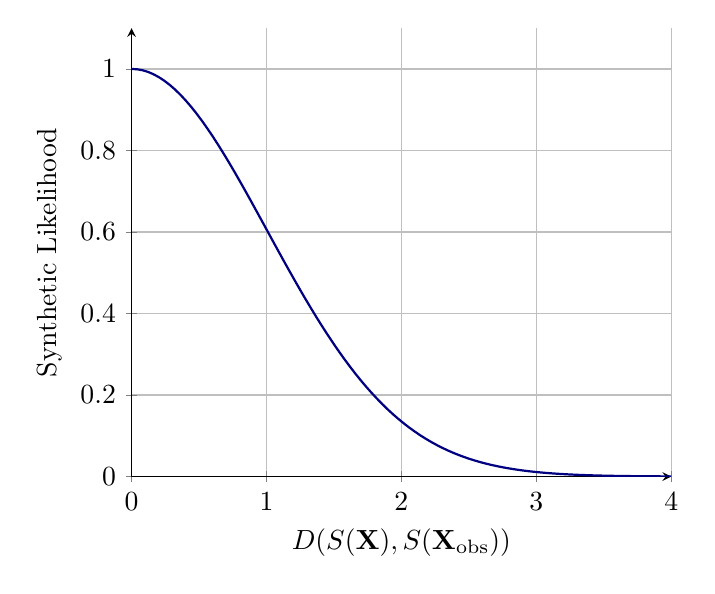
\begin{tikzpicture}
            \begin{axis}[
                    xlabel={$D(S(\mathbf{X}), S(\mathbf{X}_\text{obs}))$},
                    ylabel={Synthetic Likelihood},
                    xmin=0, xmax=4,
                    ymin=0, ymax=1.1,
                    domain=0:4,
                    samples=100,
                    axis lines=left,
                    grid=major,
                ]

                \addplot [blue!50!black, thick] {exp(-x^2/2)};

            \end{axis}
        \end{tikzpicture}
    \end{figure}
\end{frame}

\begin{frame}
    \frametitle{Overall Idea of my Research}
    \begin{itemize}
        \item Can we predict $\mathcal{D}(\bm{\theta})$ for simulated $\bm{\theta}$?
        \item <2-> Locally, hopefully yes.
    \end{itemize}
\end{frame}

\begin{frame}
    \frametitle{Gaussian Processes}
    \begin{itemize}
        \item Random functions
        \item Common examples - Brownian motion, Ornstein Uhlenbeck process
        \item <2-> Nap time for wet-lab people
    \end{itemize}
\end{frame}

\begin{frame}
    \frametitle{Gaussian Processes on $\mathbb{R}^d$}
    \begin{definnn}[Gaussian Process]
        A collection of random variables $\{f(\mathbf{x})\}_{\mathbf{x}\in\mathbb{R}^d}$ 
        is a \emph{Gaussian process} if all finite dimensional distributions are 
        multivariate normal distributed. That is, there is a function 
        $m:\mathcal{\mathbf{x}}\to\R$ and kernel $k:\mathcal{X}\times\mathcal{X}\to \R$ 
        such that for all finite sets $\{\mathbf{x}_1, \mathbf{x}_2, \dots, \mathbf{x}_n\},$
        $$\begin{bmatrix}
                f(\mathbf{x}_1) \\ f(\mathbf{x}_2)\\ \vdots\\ f(\mathbf{x}_n)
            \end{bmatrix} \sim
            \MVN\left(\begin{bmatrix}
                m(\mathbf{x}_1) \\ m(\mathbf{x}_2)\\ \vdots\\ m(\mathbf{x}_n)
            \end{bmatrix},\, \mathbf{K}\right)$$
        where $$\mathbf{K} = \begin{bmatrix}
                k(\mathbf{x}_1, \mathbf{x}_1) & k(\mathbf{x}_1, \mathbf{x}_2) & \dots  & k(\mathbf{x}_1, \mathbf{x}_n) \\
                k(\mathbf{x}_2, \mathbf{x}_1) & \ddots                        &        & \vdots                        \\
                \vdots                        &                               & \ddots & \vdots                        \\
                k(\mathbf{x}_n, \mathbf{x}_1) & \cdots                        & \cdots & k(\mathbf{x}_n, \mathbf{x}_n)
            \end{bmatrix}$$
    \end{definnn}
\end{frame}

\begin{frame}
    \frametitle{Gaussian Process Example Realisations}
    \includegraphics[width=\textwidth]{exponentiated_ell_5_tenths.pdf}
\end{frame}

\begin{frame}
    \frametitle{Covariance Kernel Motivation}\begin{itemize}
        \item Kernel determines the amount of covariance between sets of indices.
        \item When the distance between indices is small, covariance needs to be large
    \end{itemize}
\end{frame}

\begin{frame}
    \frametitle{Common Covariance Kernels}\begin{itemize}
        \item Matern Kernel
              $$k_\nu(x, x^\prime)
                  = \sigma^2\frac{2^{1 - \nu}}{\Gamma(\nu)}
                  \left(\frac{\sqrt{2\nu}||x - x^\prime||}{\ell}\right)^\nu
                  K_\nu\left(-\frac{\sqrt{2\nu}||x - x^\prime||}{\ell}\right)$$ where $K_\nu$ is a modified Bessel function ($||\cdot||$ is the euclidean distance)
        \item $\lfloor{\nu}\rfloor$ times mean square differentiable.
        \item As $\nu\to\infty$ you get squared exponential covariance function, which results in realisations that are infinitely mean square differentiable:
              $$k(x, x^\prime) = \sigma^2\exp(-\frac{||x - x^\prime||^2}{\ell})$$
    \end{itemize}
\end{frame}

\begin{frame}
    \frametitle{}
    Time to wake up
\end{frame}

\begin{frame}
    \frametitle{Kernel Choices - Kernel Type}
    \only<1>{\includegraphics[width=\textwidth]{maternonehalf_kernel.pdf}}
    \only<2>{\includegraphics[width=\textwidth]{maternthreehalves_kernel.pdf}}
    \only<3>{\includegraphics[width=\textwidth]{maternfivehalves_kernel.pdf}}
    \only<4>{\includegraphics[width=\textwidth]{exponentiated_kernel.pdf}}
\end{frame}

% \begin{frame}
%     \frametitle{Kernel Choices - length scale}
%     \only<1>{
%         $$k(x, x^\prime) = \sigma^2\exp(-\frac{||x - x^\prime||^2}{\ell})$$
%     }
%     \only<2>{\includegraphics[width=\textwidth]{exponentiated_GP_ell_5_tenths.pdf}}
%     \only<3>{\includegraphics[width=\textwidth]{exponentiated_GP_ell_10_tenths.pdf}}
%     \only<4>{\includegraphics[width=\textwidth]{exponentiated_GP_ell_20_tenths.pdf}}
% \end{frame}

\begin{frame}
    \frametitle{Fitting our GP to data}
    GPs are 'priors'
    \only<2>{\includegraphics[width=\textwidth]{flatish_GP_bare.pdf}}
    \only<3>{\includegraphics[width=\textwidth]{flatish_GP_ell_5_tenths.pdf}}
    % \only<4>{\includegraphics[width=\textwidth]{flatish_GP_ell_10_tenths.pdf}}
    % \only<5>{\includegraphics[width=\textwidth]{flatish_GP_ell_20_tenths.pdf}}
    \only<6>{\includegraphics[width=\textwidth]{flatish_GP_matern_5.0_tenths.pdf}}
    % \only<7>{\includegraphics[width=\textwidth]{flatish_GP_matern_15.0_tenths.pdf}}
    \only<8>{\includegraphics[width=\textwidth]{flatish_GP_matern_25.0_tenths.pdf}}
\end{frame}

\begin{frame}
    \frametitle{GP regression on $x(x-1)(x+1)$}
    \only<2>{\includegraphics[width=\textwidth]{cub_GP_1_iters.pdf}}
    \only<3>{\includegraphics[width=\textwidth]{cub_GP_2_iters.pdf}}
    \only<4>{\includegraphics[width=\textwidth]{cub_GP_4_iters.pdf}}
    \only<5>{\includegraphics[width=\textwidth]{cub_GP_8_iters.pdf}}
    \only<6>{\includegraphics[width=\textwidth]{cub_GP_10_iters.pdf}}
\end{frame}

\begin{frame}
    \frametitle{What if we have noise?}
    Add observation variance $\sigma^2$, $$\begin{bmatrix}
            f(\mathbf{x}_1) \\ f(\mathbf{x}_2)\\ \vdots\\ f(\mathbf{x}_n)
        \end{bmatrix} \sim
        \MVN\left(\begin{bmatrix}
            m(\mathbf{x}_1) \\ m(\mathbf{x}_2)\\ \vdots\\ m(\mathbf{x}_n)
        \end{bmatrix},\, \mathbf{K} + \sigma^2\mathbf{I}_n\right)$$
\end{frame}

\begin{frame}
    \frametitle{GP regression on $x(x-1)(x+1)$}
    % \only<2>{\includegraphics[width=\textwidth]{cub_GP_err_1_iters.pdf}}
    % \only<3>{\includegraphics[width=\textwidth]{cub_GP_err_2_iters.pdf}}
    % \only<4>{\includegraphics[width=\textwidth]{cub_GP_err_4_iters.pdf}}
    % \only<5>{\includegraphics[width=\textwidth]{cub_GP_err_8_iters.pdf}}
    \only<2>{\includegraphics[width=\textwidth]{cub_GP_err_10_iters.pdf}}
\end{frame}

\begin{frame}
    \frametitle{Overall Idea again}
    \begin{itemize}
        \item Can we predict $\mathcal{D}(\bm{\theta})$ for simulated $\bm{\theta}$
              \only<2>{\item $\mathcal{D}(\bm{\theta}) \approx \mathcal{D}(\bm{\theta}^\prime)$ for $\bm{\theta}$, $\bm{\theta}$ close.}
              \only<3>{\item Use Gaussian process to predict discrepency function}
    \end{itemize}
\end{frame}

\begin{frame}
    \frametitle{About Vivax Malaria}
    \begin{itemize}
        \item Has dormant liver stage on top of blood stage infection
    \end{itemize}
\end{frame}

\begin{frame}
    \frametitle{Champagne Model Parameters}\begin{itemize}
        \item $\alpha:$ proportion of those infected but cleared of blood stage infections (through treatment)
        \item $\beta:$ a further proportion that are also cleared of liver stage parasites, given that they were also cleared of blood stage infection (radical cure)
        \item $\lambda:$ the rate of infection
        \item $\gamma_L:$ rate of clearance of liver stage disease
        \item $f:$ rate of relapse
        \item $r:$ rate of blood stage clearance
        \item $\delta:$ importation rate (which we assume is 0)
    \end{itemize}

\end{frame}

\begin{frame}
    \frametitle{Champagne Model Transition Rates}
    \begin{figure}[htbp]
        \centering
        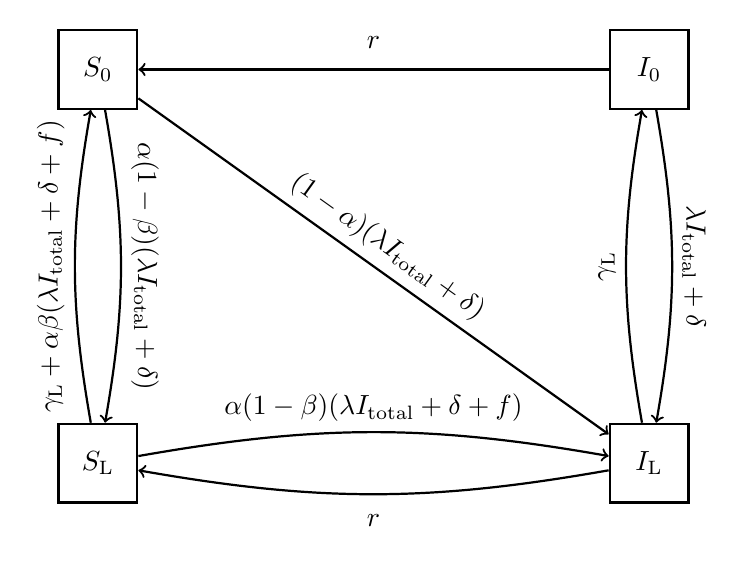
\begin{tikzpicture}[thick]
            \node[draw, minimum size=1cm] (S0) {$S_0$};
            \node[draw, right of=S0, minimum size=1cm, node distance=7cm] (I0) {$I_0$};
            \node[draw, below of=S0, minimum size=1cm, node distance=5cm] (SL) {$S_\mathrm{L}$};
            \node[draw, below of=I0, minimum size=1cm, node distance=5cm] (IL) {$I_\mathrm{L}$};
            \draw[->] (S0) edge[sloped] node[above] {$(1 - \alpha)(\lambda I_\mathrm{total} + \delta)$} (IL);
            \draw[->] (S0) edge[in = 80, out = 280, sloped] node[above] {$\alpha( 1 -\beta)(\lambda I_\mathrm{total} + \delta)$} (SL);
            \draw[->] (SL) edge[in = 260, out = 100, sloped] node [above] {$\gamma_\mathrm{L} + \alpha\beta(\lambda I_\mathrm{total} + \delta + f)$} (S0);
            \draw[->] (SL) edge[in = 170, out = 10, sloped] node [above] {$\alpha( 1 -\beta)(\lambda I_\mathrm{total} + \delta + f)$} (IL);
            \draw[->] (IL) edge[in = -10, out = 190] node [midway, label=below:{$r$}] (r) {} (SL);
            \draw[->] (IL) edge[in = 260, out = 100, sloped] node [above] {$\gamma_\mathrm{L}$} (I0);
            \draw[->] (I0) edge[in = 80, out = 280, sloped] node [above] {$\lambda I_\mathrm{total} + \delta$} (IL);
            \draw[->] (I0) edge node [midway, label=above:{$r$}] (r2) {} (S0);
        \end{tikzpicture}
        \caption{\textit{P.\ vivax} model described by \cite{champagne_using_2022}}
    \end{figure}
\end{frame}

\begin{frame}
    \frametitle{Champagne ODEs}
    \begin{align*}
        \frac{\diff I_\mathrm{L}}{\diff t} = & (1 - \alpha)(\lambda I_\mathrm{total} + \delta)(S_0 + S_\mathrm{L}) + (\lambda I_\mathrm{total} + \delta)I_0                                       \\ &  + (1 - \alpha)fS_\mathrm{L} - \gamma_\mathrm{L}I_\mathrm{L} - rI_\mathrm{L}  \\
        \frac{\diff I_0}{\diff t} =          & -(\lambda I_\mathrm{total} + \delta)I_0 + \gamma_\mathrm{L}I_\mathrm{L} - rI_0                                                                     \\
        \frac{\diff S_\mathrm{L}}{\diff t} = & -(1 - \alpha(1 - \beta))(\lambda I_\mathrm{total} + \delta + f)S_\mathrm{L} + \alpha(1-\beta)(\lambda I_\mathrm{total}                             \\ &  + \delta)S_0 - \gamma_\mathrm{L}S_\mathrm{L} + rI_\mathrm{L}       \\
        \frac{\diff S_0}{\diff t} =          & -(1 - \alpha\beta)(\lambda I_\mathrm{total} + \delta)S_0 + (\lambda I_\mathrm{total} + \delta)\alpha\beta S_\mathrm{L} + \alpha\beta fS_\mathrm{L} \\ & + \gamma_\mathrm{L}S_\mathrm{L} + rI_0
    \end{align*}
\end{frame}

\begin{frame}
    \frametitle{Model Calibration Data}\begin{itemize}
        \item Doob-Gillespie algorithm with paper parameters reported in the original paper for 'observed data', 10 initial infections, 1000 people.
        \item <2->$S(\mathbf{X}_\text{obs}) := \{w_\text{obs}, p_\text{obs}, m_\text{obs}\}$ \begin{itemize}
                  \item $w_\text{obs}:$ weekly incidence around (stochastic) equilibrium
                  \item $p_\text{obs}:$ prevalence around (stochastic) equilibrium
                  \item $m_\text{obs}:$ incidence in the first month of the epidemic
              \end{itemize}
        \item <3-> $\mathcal{D}(\bm{\theta}) := \left|\frac{w_\text{obs} - w}{w_\text{obs}}\right| + \left|\frac{p_\text{obs} - p}{p_\text{obs}}\right| + \left|\frac{m_\text{obs} - m}{m_\text{obs}}\right|$ \begin{itemize}
                  \item ($L_1$ norm on the relative differences)
              \end{itemize}
    \end{itemize}
\end{frame}

\begin{frame}
    \frametitle{Example Simulation}
    \includegraphics[width=0.95\textwidth]{doob_champagne.pdf}
\end{frame}

\begin{frame}
    \frametitle{What's the Bayesian part?}
    \begin{itemize}
        \item Bayesian acquisition function $\argmin_{\bm{\theta}}A(\bm\theta)$
        \item <2-> \cite{gutmann_bayesian_2016} uses $$\mu(\bm\theta) - \eta_t\sqrt{\mathrm{v}(\bm\theta)}$$ \begin{itemize}
                  \item $\eta_t:= \sqrt{c + 2\ln(t^{d/2 + 2})},$ and $c$ can be chosen
                  \item $\mu(\bm\theta)$ and $\mathrm{v}(\bm\theta)$ are the posterior mean and variance
              \end{itemize}
        \item <3-> Could use expected information $$(\mu_\text{min} - \mu(\bm\theta))
                  \varPhi\left(\frac{\mu_\text{min} - \mu(\bm\theta)}{\sqrt{\mathrm{v}(\bm\theta)}}\right) + \sqrt{\mathrm{v}(\bm\theta)}
                  \phi\left(\frac{\mu_\text{min} - \mu(\bm\theta)}{\sqrt{\mathrm{v}(\bm\theta)}}\right)$$\begin{itemize}
                  \item $\mu_\text{min} := \min_{\bm{\theta}} \mu(\bm\theta)$
                  \item $\varPhi, \phi$ CDF and PDF of standard normal
              \end{itemize}
    \end{itemize}
\end{frame}


\begin{frame}
    \frametitle{Acquisition `example'}
    \only<2>{\includegraphics[width=\textwidth]{cub_GP_err_10_iters.pdf}}
\end{frame}

\begin{frame}
    \frametitle{Synthetic Likelihood}
    \begin{itemize}
        \item $L(\bm\theta | \mathbf{X}_\text{obs}) \approx P(\mathcal{D}_{\mathcal{GP}}(\theta) < \varepsilon)$ (up to a proportion) where $\mathcal{D}_{\mathcal{GP}}$ is the discrepency modelled the Gaussian process
        % \item This is equivalent to using the half normal acceptance criteria
        %       \begin{figure}
        %           \centering
        %           \begin{tikzpicture}
        %               \begin{axis}[
        %                       xlabel={$D(S(\mathbf{X}), S(\mathbf{X}_\text{obs}))$},
        %                       ylabel={Synthetic Likelihood},
        %                       xmin=0, xmax=4,
        %                       ymin=0, ymax=1.1,
        %                       domain=0:4,
        %                       samples=100,
        %                       axis lines=left,
        %                       grid=major,
        %                   ]

        %                   \addplot [blue!50!black, thick] {exp(-x^2/2)};

        %               \end{axis}
        %           \end{tikzpicture}
        %       \end{figure}
    \end{itemize}
\end{frame}

\begin{frame}
    \frametitle{How did it go?}
    \only<2>{\includegraphics[width=\textwidth]{r_early.png}}
    \only<3>{\includegraphics[width=\textwidth]{r_late.png}}
    \only<4>{\includegraphics[width=\textwidth]{lambda_early.png}}
    \only<5>{\includegraphics[width=\textwidth]{lambda_late.png}}
\end{frame}

\begin{frame}
    \frametitle{Big Problem (Big Solutions?)}
    \begin{itemize}
        \item Observation variance is considered constant across the GP\begin{itemize}
                  \item Particularly a problem at the threshold
                  \item <2-> Fix by modelling observation variance as another GP
              \end{itemize}
              \item Assumes that normal distribution approximates $\mathcal{D}(\bm{\theta})$\begin{itemize}
                  \item Log-normal might be more realistic?
              \end{itemize}
              \item Jumps where there is threshold/bifurcation behaviour\begin{itemize}
                  \item Use Student $t-$Process to allow for jumps?
              \end{itemize}
    \end{itemize}
\end{frame}

\begin{frame}
    \frametitle{Thanks to}
    \begin{itemize}
        \item Eamon Conway
        \item Jennifer Flegg
        \item August for explaining GPs
    \end{itemize}
\end{frame}



\end{document}